\documentclass{standalone}
\usepackage{tikz}
\begin{document}

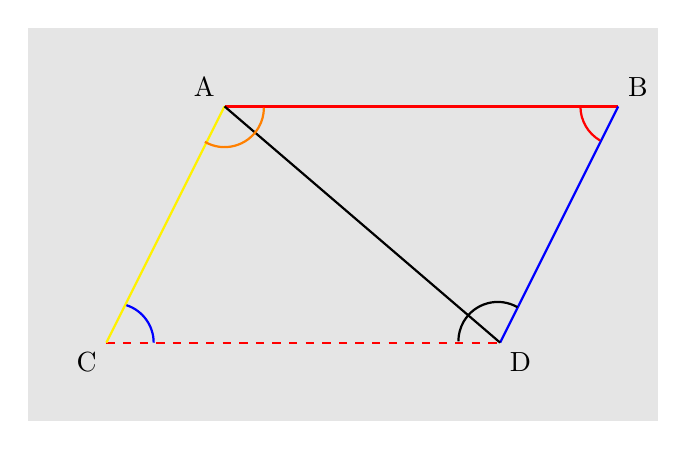
\begin{tikzpicture}

    % Set background color
    \fill[gray!20] (-1,-1) rectangle (7,4);

    % Draw parallelogram
    \draw[thick, dashed, red] (0,0) -- (5,0); % CD
    \draw[thick, yellow] (0,0) -- (1.5,3); % AC
    \draw[thick, red] (1.5,3) -- (6.5,3); % AB
    \draw[thick, blue] (6.5,3) -- (5,0); % BC
    
    % Diagonal
    \draw[thick, black] (1.5,3) -- (5,0); % AD
    
    % Vertex Labels
    \node at (0,0) [below left] {C};
    \node at (5,0) [below right] {D};
    \node at (1.5,3) [above left] {A};
    \node at (6.5,3) [above right] {B};

    % Draw angle arcs with colors
    \draw[thick, blue] (0.6,0.0) arc[start angle=0, end angle=72, radius=0.5];
    \draw[thick, orange] (1.25,2.55) arc[start angle=240, end angle=360, radius=0.5];
    \draw[thick, red] (6.02,3) arc[start angle=180, end angle=240, radius=0.5];
     \draw[thick, black] (5.22,0.45) arc[start angle=60, end angle=180, radius=0.5];
\end{tikzpicture}

\end{document}
